\documentclass[aspectratio=169,11pt]{beamer}
\usepackage[T1]{fontenc}
\usepackage{lmodern}
\usepackage{amsmath,amssymb,mathtools}
\usepackage{tikz}
\usetikzlibrary{arrows.meta,positioning,calc,fit,backgrounds,shapes.geometric}

\definecolor{famL}{RGB}{31,119,180}
\definecolor{famR}{RGB}{214,96,26}
\definecolor{zcol}{RGB}{44,140,60}
\definecolor{hcol}{RGB}{140,70,160}
\definecolor{ink}{RGB}{30,40,60}
\definecolor{soft}{RGB}{243,246,250}
\definecolor{ideabg}{RGB}{252,246,226}

\usetheme{default}
\setbeamertemplate{navigation symbols}{}
\setbeamercolor{frametitle}{fg=ink}
\setbeamerfont{frametitle}{series=\bfseries,size=\Large}
\setbeamercolor{structure}{fg=famL!80!black}
\setbeamertemplate{itemize items}[circle]
\setbeamertemplate{footline}{\hfill\color{black!45}\scriptsize\insertframenumber\,/\,\inserttotalframenumber\hspace{4mm}\vspace{2mm}}
\setbeamercolor{block title}{bg=famL!15,fg=ink}
\setbeamercolor{block body}{bg=soft}
\setbeamercolor{block title alerted}{bg=famR!20,fg=ink}
\setbeamercolor{block body alerted}{bg=ideabg}

\newcommand{\abs}[1]{\lvert #1\rvert}
\newcommand{\RR}{\mathbb R}
\newcommand{\Rf}{\mathcal R}
\newcommand{\Cf}{\mathcal C}
\newcommand{\Nout}{N^+_1}
\newcommand{\Ntwo}{N^+_2}
\newcommand{\val}{\operatorname{val}}
\newcommand{\unc}{\operatorname{unc}}
\DeclareMathOperator{\rank}{rank}
\newcommand{\cL}[1]{\textcolor{famL}{#1}}
\newcommand{\cR}[1]{\textcolor{famR}{#1}}
\newcommand{\cZ}[1]{\textcolor{zcol}{#1}}
\newcommand{\cH}[1]{\textcolor{hcol}{#1}}

\tikzset{
  vtx/.style={circle,draw,fill=white,inner sep=1.5pt,minimum size=5.5mm,font=\small},
  dot/.style={circle,fill,inner sep=1.4pt},
  arc/.style={-{Stealth[length=2.2mm]},thick},
  gridpt/.style={circle,draw=black!25,fill=white,inner sep=0pt,minimum size=2.2mm},
  Lpt/.style={circle,draw=famL!70!black,fill=famL,inner sep=0pt,minimum size=3.2mm},
  Rpt/.style={rectangle,draw=famR!70!black,fill=famR,inner sep=0pt,minimum size=3.0mm},
  Zpt/.style={diamond,draw=zcol!70!black,fill=zcol,inner sep=0pt,minimum size=3.8mm},
  Hpt/.style={star,star points=5,draw=hcol!70!black,fill=hcol,inner sep=0pt,minimum size=4.2mm},
  box/.style={draw,rounded corners,align=center,font=\small,fill=soft,minimum height=12mm,text width=33mm},
}

\title{A proof of Seymour's second-neighborhood conjecture}
\subtitle{How the proof works: three stages and one new lemma}
\author{Talk based on the OpenAI preprint (Sept.\ 23, 2026)\\[2pt]\footnotesize prepared by Claude (Opus 5.5)}
\date{}

\begin{document}

\begin{frame}
\titlepage
\end{frame}

% ------------------------------------------------------------------
\begin{frame}{The conjecture}
\begin{columns}[T]
\begin{column}{0.55\textwidth}
\emph{Oriented graph}: finite digraph, no loops, no 2-cycles $x\to y\to x$.

\medskip
$\Nout(v)$ = vertices at distance exactly $1$,\\
$\Ntwo(v)$ = vertices at distance exactly $2$.

\begin{block}{Theorem (Seymour's second-neighborhood conjecture)}
Every nonempty finite oriented graph has a vertex $v$ with
\[\abs{\Nout(v)}\le\abs{\Ntwo(v)}.\]
\end{block}
\small A \emph{Seymour vertex}. Sinks are Seymour vertices. In a directed
triangle every vertex has equality.
\end{column}
\begin{column}{0.42\textwidth}
\centering
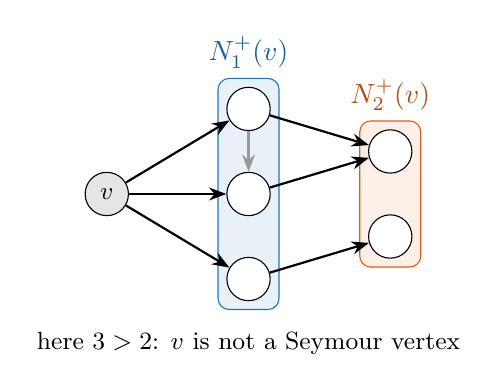
\begin{tikzpicture}[scale=0.9]
 \node[vtx,fill=black!10] (v) at (0,0) {$v$};
 \node[vtx] (u1) at (2,1.2) {}; \node[vtx] (u2) at (2,0) {}; \node[vtx] (u3) at (2,-1.2) {};
 \node[vtx] (w1) at (4,0.6) {}; \node[vtx] (w2) at (4,-0.6) {};
 \foreach \u in {u1,u2,u3} \draw[arc] (v)--(\u);
 \draw[arc] (u1)--(w1); \draw[arc] (u2)--(w1); \draw[arc] (u3)--(w2);
 \draw[arc,black!40] (u1)--(u2);
 \begin{scope}[on background layer]
  \node[draw=famL,fill=famL!10,rounded corners,fit=(u1)(u3),inner sep=3pt,label={[famL!80!black]above:$\Nout(v)$}] {};
  \node[draw=famR,fill=famR!10,rounded corners,fit=(w1)(w2),inner sep=3pt,label={[famR!80!black]above:$\Ntwo(v)$}] {};
 \end{scope}
 \node[font=\small] at (2,-2.1) {here $3>2$: $v$ is not a Seymour vertex};
\end{tikzpicture}
\end{column}
\end{columns}
\end{frame}

% ------------------------------------------------------------------
\begin{frame}{Before this proof}
\begin{itemize}
\item \textbf{Tournaments} (Dean's conjecture): Fisher 1996 (Farkas' lemma),
Havet--Thomass\'e 2000 (median orders).
\item Tournaments minus a matching / star / clique / two stars \ldots
\item Minimum outdegree $\le 6$ (Kaneko--Locke), $=7$ (computer-assisted).
\item Ratio versions: some $v$ has $\abs{\Ntwo(v)}\ge\gamma\abs{\Nout(v)}$,
$\gamma\approx0.657\to0.7155$.
\item Two tools that the proof builds on:
 \begin{itemize}
 \item minimal counterexample + \textbf{blow-up} (Brantner--Brockman--Kay--Snively 2009),
 \item the conjecture for \textbf{sets of vertices} (Seacrest).
 \end{itemize}
\end{itemize}
\end{frame}

% ------------------------------------------------------------------
\begin{frame}{The proof at a glance}
\centering
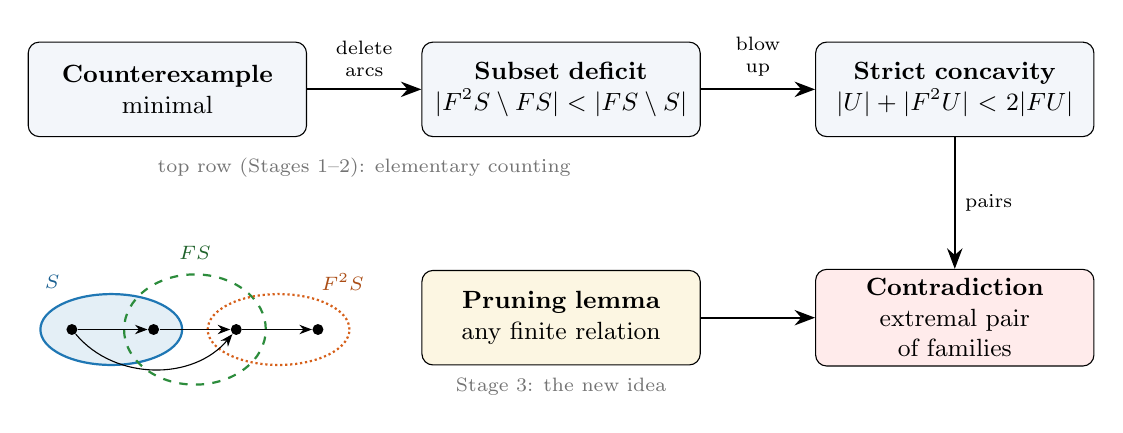
\begin{tikzpicture}[every edge/.style={draw,-{Stealth[length=2.6mm]},thick},
  lab/.style={font=\scriptsize,align=center}]
 \node[box] (ce) at (0,0) {\textbf{Counterexample}\\ minimal};
 \node[box] (sd) at (5.0,0) {\textbf{Subset deficit}\\ $\abs{F^2S\setminus FS}<\abs{FS\setminus S}$};
 \node[box] (cc) at (10.0,0) {\textbf{Strict concavity}\\ $\abs U+\abs{F^2U}<2\abs{FU}$};
 \node[box,fill=ideabg] (pr) at (5.0,-2.9) {\textbf{Pruning lemma}\\ any finite relation};
 \node[box,fill=red!8] (con) at (10.0,-2.9) {\textbf{Contradiction}\\ extremal pair of families};
 \draw (ce) edge node[lab,above=1pt] {delete\\arcs} (sd);
 \draw (sd) edge node[lab,above=1pt] {blow\\up} (cc);
 \draw (cc) edge node[lab,right] {pairs} (con);
 \draw (pr) edge (con);
 \node[font=\scriptsize,text=black!55] at (2.5,-1.0) {top row (Stages 1--2): elementary counting};
 \node[font=\scriptsize,text=black!55,below=1pt] at (pr.south) {Stage 3: the new idea};
 % mini-sketch of F(S) and F^2(S)
 \begin{scope}[shift={(0.35,-3.05)},scale=1.25]
  \draw[famL,thick,fill=famL!12] (-0.85,0) ellipse (0.72 and 0.36);
  \draw[zcol,thick,dashed] (0,0) ellipse (0.72 and 0.56);
  \draw[famR,thick,densely dotted] (0.85,0) ellipse (0.72 and 0.36);
  \node[dot] (s1) at (-1.25,0) {}; \node[dot] (s2) at (-0.42,0) {};
  \node[dot] (u) at (0.42,0) {};   \node[dot] (w) at (1.25,0) {};
  \draw[-{Stealth[length=1.6mm]}] (s1)--(s2);
  \draw[-{Stealth[length=1.6mm]}] (s2)--(u);
  \draw[-{Stealth[length=1.6mm]}] (u)--(w);
  \draw[-{Stealth[length=1.6mm]}] (s1) to[bend right=50] (u);
  \node[font=\scriptsize,famL!80!black] at (-1.45,0.48) {$S$};
  \node[font=\scriptsize,zcol!70!black] at (0,0.78) {$FS$};
  \node[font=\scriptsize,famR!80!black] at (1.5,0.48) {$F^2S$};
 \end{scope}
\end{tikzpicture}

\medskip
\small Notation: $FS=F(S)=\{y: x\to y \text{ for some } x\in S\}$ (one step; may meet $S$),\\
$F^2S=F(F(S))$ (exactly two steps), \quad so\quad $\Ntwo(v)=F^2\{v\}\setminus F\{v\}$.
\end{frame}

% ------------------------------------------------------------------
\begin{frame}{Stage 1: from one vertex to all sets}
\begin{block}{Lemma (subset deficit)}
In a counterexample with fewest vertices, then fewest arcs,
\[\abs{F^2(S)\setminus F(S)}<\abs{F(S)\setminus S}\qquad\text{for all }\varnothing\ne S\subsetneq V.\]
\end{block}
\begin{columns}[T]
\begin{column}{0.56\textwidth}
\small
For $S=\{v\}$ this is just ``$v$ is not a Seymour vertex''.

\medskip
\textbf{Why fewest vertices first?} The minimal counterexample is strongly
connected (a sink component would be a smaller one), so $F(S)\setminus S\ne\varnothing$.

\medskip
\textbf{Why fewest arcs?} Deleting arcs gives a graph that \emph{has} a
Seymour vertex, and we can analyze what that vertex lost.
\end{column}
\begin{column}{0.42\textwidth}
\centering
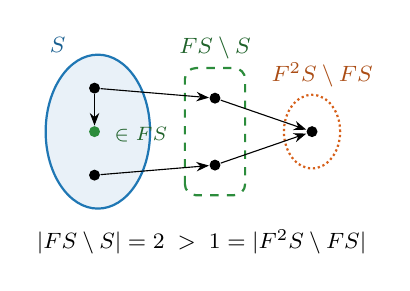
\begin{tikzpicture}[scale=0.85,a/.style={-{Stealth[length=1.6mm]}}]
 \draw[famL,thick,fill=famL!10] (0.05,0) ellipse (0.78 and 1.15);
 \draw[zcol,thick,dashed,rounded corners] (1.35,-0.95) rectangle (2.25,0.95);
 \draw[famR,thick,densely dotted] (3.25,0) ellipse (0.42 and 0.55);
 \node[dot] (a) at (0,0.65) {};
 \node[dot,fill=zcol] (b) at (0,0) {};
 \node[dot] (c) at (0,-0.65) {};
 \node[dot] (e1) at (1.8,0.5) {}; \node[dot] (e2) at (1.8,-0.5) {};
 \node[dot] (f) at (3.25,0) {};
 \draw[a] (a)--(b); \draw[a] (a)--(e1); \draw[a] (c)--(e2);
 \draw[a] (e1)--(f); \draw[a] (e2)--(f);
 \node[font=\footnotesize,famL!80!black] at (-0.55,1.3) {$S$};
 \node[font=\footnotesize,zcol!70!black] at (1.8,1.25) {$FS\setminus S$};
 \node[font=\footnotesize,famR!80!black] at (3.4,0.85) {$F^2S\setminus FS$};
 \node[font=\scriptsize,zcol!70!black,anchor=west] at (0.15,-0.05) {$\in FS$};
 \node[font=\footnotesize,align=center] at (1.6,-1.65) {$\abs{FS\setminus S}=2\;>\;1=\abs{F^2S\setminus FS}$};
\end{tikzpicture}
\end{column}
\end{columns}
\end{frame}

% ------------------------------------------------------------------
\begin{frame}{Stage 1: proving the subset deficit}
\begin{block}{Goal: for a fixed nonempty proper $S$, show $\abs{F^2S\setminus FS}<\abs{FS\setminus S}$}
\small Idea: add $E=FS\setminus S$ in batches $Q$; each batch adds \emph{fewer than} $\abs Q$ new two-step vertices.
\end{block}
\vspace{-2pt}
\begin{columns}[c]
\begin{column}{0.41\textwidth}
\centering
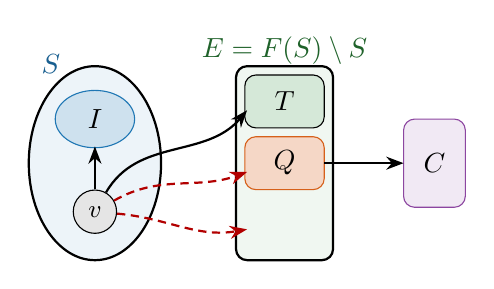
\begin{tikzpicture}[scale=0.56]
 \draw[thick,fill=famL!8] (0,0) ellipse (1.5 and 2.2);
 \node[famL!80!black] at (-1.0,2.25) {$S$};
 \draw[fill=famL!22,draw=famL] (0,1.0) ellipse (0.9 and 0.65); \node at (0,1.0) {$I$};
 \node[vtx,fill=black!10] (v) at (0,-1.1) {$v$};
 \draw[thick,rounded corners,fill=zcol!7] (3.2,-2.2) rectangle (5.4,2.2);
 \node[zcol!70!black] at (4.3,2.55) {$E=F(S)\setminus S$};
 \draw[rounded corners,fill=zcol!20] (3.4,0.8) rectangle (5.2,2.0); \node at (4.3,1.4) {$T$};
 \draw[rounded corners,fill=famR!25,draw=famR] (3.4,-0.6) rectangle (5.2,0.6); \node at (4.3,0) {$Q$};
 \draw[rounded corners,fill=hcol!12,draw=hcol] (7.0,-1.0) rectangle (8.4,1.0); \node at (7.7,0) {$C$};
 \draw[arc,red!70!black,densely dashed] (v) to[out=30,in=200] (3.45,-0.2);
 \draw[arc,red!70!black,densely dashed] (v) to[out=-5,in=190] (3.45,-1.5);
 \draw[arc] (v) to[out=60,in=230] (3.45,1.2);
 \draw[arc] (v) -- (0,0.38);
 \draw[arc] (5.2,0) -- (7.0,0);
\end{tikzpicture}
\end{column}
\begin{column}{0.57\textwidth}
\small
\begin{itemize}\setlength{\itemsep}{2pt}
\item $I=FS\cap S$. Progress counter for $T\subseteq E$:
$g(T)=\abs{F(T)\setminus(I\cup T)}$, the \emph{new} vertices reached from $T$.
$g(\varnothing)=0$ and $g(E)=\abs{F^2S\setminus FS}$.
\item Grow $T$ from $\varnothing$ to $E$; each time, delete all arcs $S\to E\setminus T$.
\item Fewer arcs $\Rightarrow$ a Seymour vertex $v$. It must be in $S$ and lose
its out-neighbors $Q\subseteq E\setminus T$.
\item $v$ \emph{loses} $C$ (reached only via $Q$) and gains $\le\abs{Q\cap F(T)}$.
Since $v$ was \emph{not} Seymour in $D$,
$g(T\cup Q)-g(T)<\abs Q$.
\item Sum: $\abs{F^2S\setminus FS}=g(E)<\abs E=\abs{FS\setminus S}$.
\end{itemize}
\end{column}
\end{columns}
\end{frame}

% ------------------------------------------------------------------
\begin{frame}{Stage 2: drowning the error term}
We want a quantity that \emph{adds up} over many sets:
\[
 \kappa(S)=\abs S-2\abs{FS}+\abs{F^2S}\ \le\ \underbrace{\bigl(\abs{F^2S\setminus FS}-\abs{FS\setminus S}\bigr)}_{\le-1\text{ by Stage 1}}+\underbrace{\abs{S\setminus FS}}_{\text{error}}.
\]
\begin{columns}[c]
\begin{column}{0.48\textwidth}
\textbf{Blow-up} $G=D[T_m]$: each vertex becomes a transitive tournament
on $m>n$ vertices.
\begin{itemize}
\item main term $\times m$,
\item error $\le1$ per block, since $\abs{\tau(T)}\ge\abs T-1$ ($\tau$: forward image in $T_m$).
\end{itemize}
Result: $\kappa_G(U)\le -m+n<0$ when the support of $U$ is proper\\ {\small(the other case is immediate).}
\end{column}
\begin{column}{0.48\textwidth}
\centering
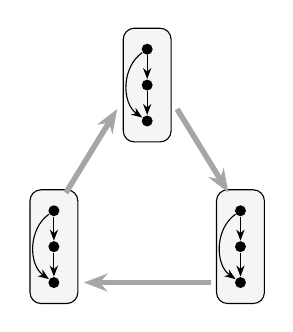
\begin{tikzpicture}[scale=0.76]
  \foreach \nm/\ang in {x/90,y/210,z/330}{
   \begin{scope}[shift={(\ang:1.8)}]
    \draw[rounded corners,fill=black!4] (-0.4,-0.95) rectangle (0.4,0.95);
    \node[dot] (\nm1) at (0,0.6) {}; \node[dot] (\nm2) at (0,0) {}; \node[dot] (\nm3) at (0,-0.6) {};
    \draw[-{Stealth[length=1.4mm]}] (\nm1)--(\nm2); \draw[-{Stealth[length=1.4mm]}] (\nm2)--(\nm3);
    \draw[-{Stealth[length=1.4mm]}] (\nm1) to[bend right=55] (\nm3);
   \end{scope}}
  \draw[-{Stealth[length=3mm]},line width=2pt,black!35] ($(90:1.8)+(0.5,-0.4)$) -- ($(330:1.8)+(-0.2,0.9)$);
  \draw[-{Stealth[length=3mm]},line width=2pt,black!35] ($(330:1.8)+(-0.5,-0.6)$) -- ($(210:1.8)+(0.5,-0.6)$);
  \draw[-{Stealth[length=3mm]},line width=2pt,black!35] ($(210:1.8)+(0.2,0.9)$) -- ($(90:1.8)+(-0.5,-0.4)$);
\end{tikzpicture}
\end{column}
\end{columns}
\end{frame}

% ------------------------------------------------------------------
\begin{frame}{After Stages 1--2}
\begin{block}{Done so far}
If the theorem fails: a minimal counterexample $D$ has the subset deficit
(Stage~1), and its blow-up $G=D[T_m]$ satisfies (G1), (G2) below (Stage~2).
\end{block}
\begin{alertblock}{What remains to show (Stage 3; this finishes the proof)}
There is no nonempty oriented graph $G$ such that
\begin{itemize}
\item[(G1)] every vertex has an in-neighbor, and
\item[(G2)] every nonempty proper $U\subseteq V(G)$ is \emph{strictly concave}:
$\abs U+\abs{F^2U}<2\abs{FU}$,\\ i.e.\ $\abs U,\ \abs{FU},\ \abs{F^2U}$ has
a smaller second increment than its first.
\end{itemize}
\end{alertblock}
Single sets will not give a contradiction. Instead we look at
\textbf{families of pairs of vertices} and apply (G2) to all of their
rows and columns at once.
\end{frame}

% ------------------------------------------------------------------
\begin{frame}{Stage 3: the grid $X\times X$}
\begin{block}{Aim of Stage 3: no $G$ with (G1), (G2) exists}
Plan: work with sets of \emph{pairs} of vertices, choose the ``best'' pair
of such sets, and use (G2) to build a better one. Contradiction.\\
\emph{This slide:} the setting, and why (G2) still applies to sets of pairs.
\end{block}
\begin{columns}[c]
\begin{column}{0.52\textwidth}
\small
$X=V(G)$; pair $(i,j)$: row $i$, column $j$.
\begin{itemize}
\item $F_1$: move the \textbf{first} coordinate along an arc (vertical);
\item $F_2$: move the \textbf{second} coordinate along an arc (horizontal).
\end{itemize}
Line by line: $(F_1P)_j=F(P_j)$ for every column $P_j$. So if every column
of $P$ is nonempty and proper, (G2) column by column gives
\[\abs P+\abs{F_1^2P}<2\abs{F_1P}.\]
\end{column}
\begin{column}{0.45\textwidth}
\centering
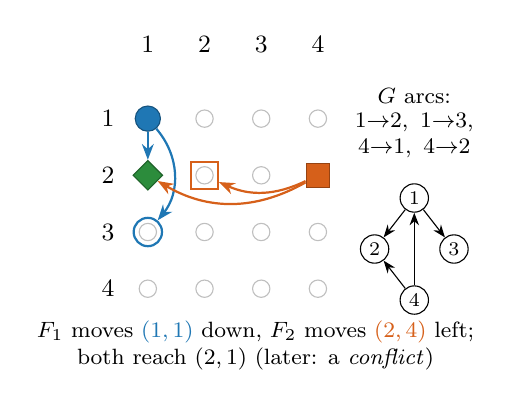
\begin{tikzpicture}[scale=0.72]
  \foreach \k in {1,...,4} {\node[font=\small] at (\k,-0.3) {$\k$}; \node[font=\small] at (0.3,-\k-0.6) {$\k$};}
  \foreach \i in {1,...,4} \foreach \j in {1,...,4} \node[gridpt] at (\j,-\i-0.6) {};
  \node[Lpt] (r) at (1,-1.6) {}; \node[Rpt] (c) at (4,-2.6) {}; \node[Zpt] (z) at (1,-2.6) {};
  \node[circle,draw=famL,thick,inner sep=0pt,minimum size=3.6mm] (r3) at (1,-3.6) {};
  \node[rectangle,draw=famR,thick,inner sep=0pt,minimum size=3.4mm] (c2) at (2,-2.6) {};
  \draw[-{Stealth[length=2mm]},famL,thick] (r) -- (z);
  \draw[-{Stealth[length=2mm]},famL,thick] (r) to[bend left=40] (r3);
  \draw[-{Stealth[length=2mm]},famR,thick] (c) to[bend left=25] (c2);
  \draw[-{Stealth[length=2mm]},famR,thick] (c) to[bend left=30] (z);
  \node[font=\footnotesize] at (5.7,-1.2) {$G$ arcs:};
  \node[font=\footnotesize,align=center] at (5.7,-1.9) {$1{\to}2,\ 1{\to}3$,\\ $4{\to}1,\ 4{\to}2$};
  \begin{scope}[every node/.style={circle,draw,inner sep=0pt,minimum size=3.6mm,font=\scriptsize}]
   \node (g1) at (5.7,-3.0) {1}; \node (g2) at (5.0,-3.9) {2};
   \node (g3) at (6.4,-3.9) {3}; \node (g4) at (5.7,-4.8) {4};
  \end{scope}
  \draw[-{Stealth[length=1.6mm]}] (g1)--(g2); \draw[-{Stealth[length=1.6mm]}] (g1)--(g3);
  \draw[-{Stealth[length=1.6mm]}] (g4)--(g1); \draw[-{Stealth[length=1.6mm]}] (g4)--(g2);
  \node[font=\footnotesize,align=center] at (2.9,-5.6) {$F_1$ moves {\color{famL}$(1,1)$} down,
    $F_2$ moves {\color{famR}$(2,4)$} left;\\ both reach $(2,1)$ (later: a \emph{conflict})};
\end{tikzpicture}
\end{column}
\end{columns}
\end{frame}

% ------------------------------------------------------------------
\begin{frame}{Conflicts and compatibility}
\begin{block}{Goal: say which pairs of families $(P,Q)$ Stage 3 is allowed to use}
Stage 3 uses a \emph{left} family $P\subseteq X\times X$, moved vertically by
$F_1$, and a \emph{right} family $Q$, moved horizontally by $F_2$. It only
allows pairs $(P,Q)$ whose images never meet (\emph{compatible}) and picks the
best one.
\end{block}
\begin{columns}[c]
\begin{column}{0.55\textwidth}
A left member $\cL{r=(p,j)}\in P$ and a right member $\cR{c=(i,s)}\in Q$
\textbf{conflict} if $p\to i$ and $s\to j$ in $G$,
i.e.\ their images $F_1\{r\}$, $F_2\{c\}$ meet, at $\cZ{z=(i,j)}$.

\smallskip
$(P,Q)$ is \textbf{compatible} if there is no conflict:
$F_1P\cap F_2Q=\varnothing$.

\smallskip
Every conflict spans a rectangle. Its fourth corner $\cH{h=(p,s)}$ will be
important.
\end{column}
\begin{column}{0.42\textwidth}
\centering
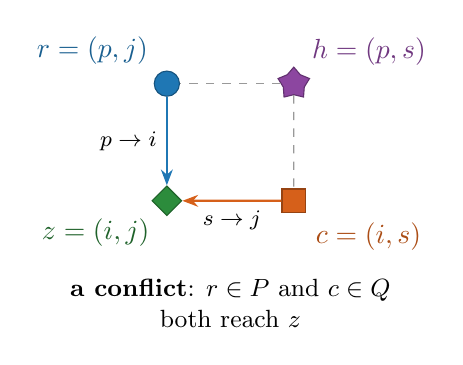
\begin{tikzpicture}[scale=0.62]
  \node[Lpt,label={[famL!80!black]above left:$r=(p,j)$}] (rr) at (0,0) {};
  \node[Hpt,label={[hcol!80!black]above right:$h=(p,s)$}] (h) at (2.6,0) {};
  \node[Zpt,label={[zcol!70!black]below left:$z=(i,j)$}] (zz) at (0,-2.4) {};
  \node[Rpt,label={[famR!80!black]below right:$c=(i,s)$}] (cc) at (2.6,-2.4) {};
  \draw[-{Stealth[length=2mm]},thick,famL] (rr) -- node[left,font=\footnotesize,black] {$p\to i$} (zz);
  \draw[-{Stealth[length=2mm]},thick,famR] (cc) -- node[below,font=\footnotesize,black] {$s\to j$} (zz);
  \draw[black!40,dashed] (h)--(rr); \draw[black!40,dashed] (h)--(cc);
  \node[font=\small,align=center] at (1.3,-4.5) {\textbf{a conflict}: $r\in P$ and $c\in Q$\\ both reach $z$};
\end{tikzpicture}
\end{column}
\end{columns}
\end{frame}

% ------------------------------------------------------------------
\begin{frame}{The extremal set-up}
\textbf{Goal:} choose a quantity to maximize, so that a maximizer gives a contradiction.

\medskip
$P,Q\subseteq X\times X$ are just two \textbf{sets of grid points} (pairs of
vertices); $P$ is moved by $F_1$, $Q$ by $F_2$.
\begin{block}{$(P,Q)$ is admissible if}
(a) no conflict: $F_1P\cap F_2Q=\varnothing$, and\\
(b) both contain the diagonal $\Delta=\{(v,v):v\in X\}$.
\end{block}
{\small\textbf{Example:} $(\Delta,\Delta)$ is admissible. (b) is clear. $F_1\Delta=\{(i,j):j\to i\}$,
$F_2\Delta=\{(i,j):i\to j\}$, and a common point would need $i\to j$ and $j\to i$:
impossible in an oriented graph. So admissible pairs exist.\par}

\medskip
\textbf{Objective:}\quad $\val(P,Q)=\abs P+\abs Q+\unc(P,Q)$,\\
$\unc=\#$points covered by neither $F_1P$ nor $F_2Q$.

\medskip
Take an admissible $(P,Q)$ of \textbf{maximum value}; $\mu=\abs P+\abs Q$, $d=\unc$.\\
\textbf{Next:} build an admissible $(P',Q')$ with larger value. Contradiction.
\end{frame}

% ------------------------------------------------------------------
\begin{frame}{The improvement step}
New families, as complements of the \textbf{second} images (note the swap):
\[
 \cL{\Rf}=(X\times X)\setminus F_2^2Q,\qquad \cR{\Cf}=(X\times X)\setminus F_1^2P.
\]
{\small $\cH H$ = set of \emph{opposite corners}: for each conflict of $r=(p,j)\in\Rf$ with
$c=(i,s)\in\Cf$, the corner $\cH{h=(p,s)}$ of its rectangle (opposite to the meeting point $z=(i,j)$, slide~10).}
\begin{itemize}
\item \textbf{Gain.} Concavity on all lines:\quad $\abs\Rf+\abs\Cf>\mu+2d$.
\item \textbf{The diagonal survives} and is conflict-free.
\item \textbf{Opposite corners were uncovered.}\quad $H\cap(F_1P\cup F_2Q)=\varnothing$,\quad so $\abs H\le d$.
\end{itemize}
\begin{columns}[c]
\begin{column}{0.42\textwidth}
\small All three are \emph{two-step path} arguments. For example, if $h\in F_1P$ via
$(u,s)\in P$, then one more step down puts $c$ in $F_1^2P$. But
$c\in\Cf$, the complement.
\end{column}
\begin{column}{0.56\textwidth}
\centering
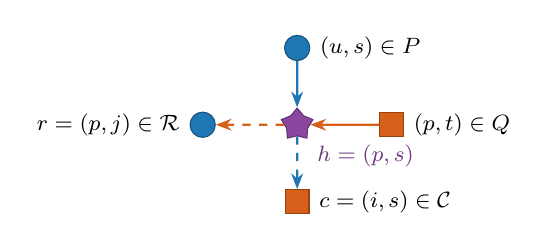
\begin{tikzpicture}[scale=0.75]
  \node[Lpt,label={[font=\footnotesize]right:$(u,s)\in P$}] (us) at (1.6,0) {};
  \node[Hpt,label={[font=\footnotesize,hcol!80!black]below right:$h=(p,s)$}] (h) at (1.6,-1.3) {};
  \node[Rpt,label={[font=\footnotesize]right:$c=(i,s)\in\Cf$}] (c) at (1.6,-2.6) {};
  \node[Rpt,label={[font=\footnotesize]right:$(p,t)\in Q$}] (pt) at (3.2,-1.3) {};
  \node[Lpt,label={[font=\footnotesize]left:$r=(p,j)\in\Rf$}] (r) at (0,-1.3) {};
  \draw[-{Stealth[length=2mm]},thick,famL] (us) -- (h);
  \draw[-{Stealth[length=2mm]},thick,famL,dashed] (h) -- (c);
  \draw[-{Stealth[length=2mm]},thick,famR] (pt) -- (h);
  \draw[-{Stealth[length=2mm]},thick,famR,dashed] (h) -- (r);
\end{tikzpicture}
\end{column}
\end{columns}
\end{frame}

% ------------------------------------------------------------------
\begin{frame}{The new ingredient: the pruning lemma}
\begin{alertblock}{Pruning lemma (any finite relation $\to$ on $X$, any $\Rf,\Cf\subseteq X\times X$)}
One can delete members so that no conflicts remain, keeping every member
that was in no conflict, with
\[
 \#\text{deleted}\ \le\ \abs{\cH H}+\#\{z\in \cZ Z:\ z\text{ uncovered \emph{after} pruning}\}.
\]
\end{alertblock}
\begin{itemize}
\item $\cZ Z$ = conflict points, $\cH H$ = opposite corners of conflicts.
\item After pruning to $\Rf'\subseteq\Rf$, $\Cf'\subseteq\Cf$, a point is \textbf{uncovered} if no
kept member reaches it: it is not in $F_1\Rf'\cup F_2\Cf'$. Only points of $\cZ Z$ are
counted. Before pruning each $z\in\cZ Z$ is covered (by both members of its
conflict), so these are exactly the conflict points that pruning uncovered.
\item The cost depends on the \textbf{outcome} of the pruning, not only on the input.
\item No orientation is used: this is a statement about arbitrary relations.
\end{itemize}
\end{frame}

% ------------------------------------------------------------------
\begin{frame}{An exchange rate, not a minimum}
\begin{columns}[c]
\begin{column}{0.44\textwidth}
\centering
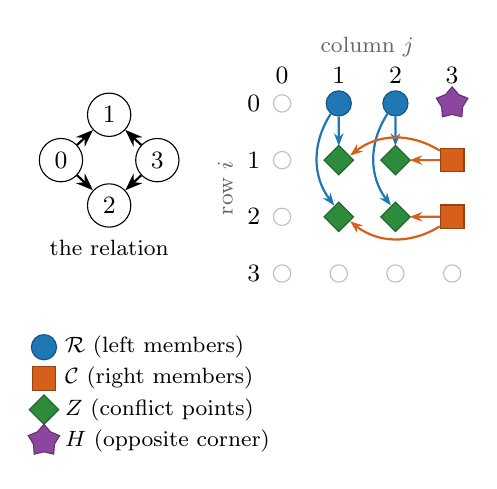
\begin{tikzpicture}[scale=0.72]
  \begin{scope}[xshift=-3.9cm,yshift=-1.0cm]
  \node[vtx] (x0) at (0,0) {$0$}; \node[vtx] (x3) at (1.7,0) {$3$};
  \node[vtx] (x1) at (0.85,0.8) {$1$}; \node[vtx] (x2) at (0.85,-0.8) {$2$};
  \draw[arc] (x0)--(x1); \draw[arc] (x0)--(x2); \draw[arc] (x3)--(x1); \draw[arc] (x3)--(x2);
  \end{scope}
  \node[font=\footnotesize] at (-3.05,-2.55) {the relation};
  \node[font=\footnotesize,text=black!60] at (1.5,1.0) {column $j$};
  \node[font=\footnotesize,text=black!60,rotate=90] at (-1.0,-1.5) {row $i$};
  \foreach \k in {0,1,2,3} {\node[font=\small] at (\k,0.5) {$\k$}; \node[font=\small] at (-0.5,-\k) {$\k$};}
  \foreach \i in {0,...,3} \foreach \j in {0,...,3} \node[gridpt] at (\j,-\i) {};
  \foreach \i in {1,2} \foreach \j in {1,2} \node[Zpt] at (\j,-\i) {};
  \node[Hpt] at (3,0) {};
  \node[Lpt] (r1) at (1,0) {}; \node[Lpt] (r2) at (2,0) {};
  \node[Rpt] (c1) at (3,-1) {}; \node[Rpt] (c2) at (3,-2) {};
  \draw[famL,-{Stealth[length=1.6mm]},thick] (r1)--(1,-0.75);
  \draw[famL,-{Stealth[length=1.6mm]},thick] (r2)--(2,-0.75);
  \draw[famR,-{Stealth[length=1.6mm]},thick] (c1)--(2.25,-1);
  \draw[famR,-{Stealth[length=1.6mm]},thick] (c2)--(2.25,-2);
  \draw[famL,-{Stealth[length=1.6mm]},thick] (r1) to[bend right=35] (0.92,-1.8);
  \draw[famL,-{Stealth[length=1.6mm]},thick] (r2) to[bend right=35] (1.92,-1.8);
  \draw[famR,-{Stealth[length=1.6mm]},thick] (c1) to[bend right=35] (1.2,-0.92);
  \draw[famR,-{Stealth[length=1.6mm]},thick] (c2) to[bend left=35] (1.2,-2.08);
  \begin{scope}[yshift=-4.3cm,xshift=-4.2cm,font=\footnotesize]
   \node[Lpt] at (0,0) {}; \node[anchor=west] at (0.2,0) {$\Rf$ (left members)};
   \node[Rpt] at (0,-0.55) {}; \node[anchor=west] at (0.2,-0.55) {$\Cf$ (right members)};
   \node[Zpt] at (0,-1.1) {}; \node[anchor=west] at (0.2,-1.1) {$Z$ (conflict points)};
   \node[Hpt] at (0,-1.65) {}; \node[anchor=west] at (0.2,-1.65) {$H$ (opposite corner)};
  \end{scope}
\end{tikzpicture}
\end{column}
\begin{column}{0.54\textwidth}
\small
$\Rf=\{01,02\}$, $\Cf=\{13,23\}$ (pair $ij$ = row $i$, column $j$); arcs $0\to1,\,0\to2,\,3\to1,\,3\to2$.
Arrows: what each member covers.
\begin{itemize}
\item All $4$ pairs conflict; $\abs Z=4$, $\abs H=1$.
\item Cheapest pruning: delete one side ($2$ deletions). But then all of $Z$
stays covered, and $2>\abs H+0$.
\item Delete all $4$: then all $4$ points of $Z$ are uncovered, and $4\le1+4$. \checkmark
\end{itemize}
\textbf{Moral:} extra deletions are allowed if they are paid for with
uncovered points. In our objective, uncovered points are worth exactly as
much as members.
\end{column}
\end{columns}
\end{frame}

% ------------------------------------------------------------------
\begin{frame}{The ledger closes up}
Prune $(\Rf,\Cf)$ to $(P',Q')$, admissible, with $d'=\unc(P',Q')$:
\begin{align*}
 \val(P',Q')&=\underbrace{\abs{P'}+\abs{Q'}}_{\ge\,\abs\Rf+\abs\Cf-\abs H-d'}
 +\underbrace{\unc(P',Q')}_{=\,d'}\\
 &\ge\ \abs\Rf+\abs\Cf-\abs H\ >\ \mu+2d-d=\val(P,Q).
\end{align*}
{\small\textbf{Why $-d'$?} The pruning lemma allows $\abs H$ deletions plus one per
conflict point left uncovered, and those are among the $d'$ uncovered points.
\textbf{Why $+d'$?} It is the $\unc$ term in the definition of $\val$: uncovered
points count like members, so those deletions are paid back exactly.\par}
\medskip
\begin{columns}[c]
\begin{column}{0.5\textwidth}
Contradiction with maximality, so \textbf{no strictly concave graph exists}
and the theorem follows.

\medskip
\small Why weight $1$ on $\unc$? With weight $\lambda$ the bound becomes
$\mu+d+(\lambda-1)d'$, to be compared with $\mu+\lambda d$. Only $\lambda=1$
always works.
\end{column}
\begin{column}{0.48\textwidth}
\centering
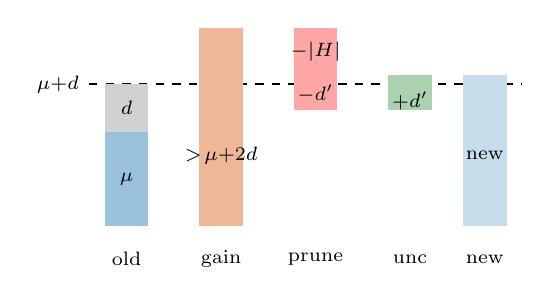
\begin{tikzpicture}[yscale=0.3,xscale=0.5]
 \draw[dashed,thick] (-0.4,6) node[left,font=\scriptsize] {$\mu{+}d$} --(10.6,6);
 \fill[famL!45] (0,0) rectangle (1.1,4); \fill[black!18] (0,4) rectangle (1.1,6);
 \fill[famR!45] (2.4,0) rectangle (3.5,8.4);
 \fill[red!35] (4.8,4.9) rectangle (5.9,8.4);
 \fill[zcol!40] (7.2,4.9) rectangle (8.3,6.4);
 \fill[famL!25] (9.1,0) rectangle (10.2,6.4);
 \node[font=\scriptsize] at (0.55,2) {$\mu$}; \node[font=\scriptsize] at (0.55,5) {$d$};
 \node[font=\scriptsize] at (2.95,3) {$>\!\mu{+}2d$};
 \node[font=\scriptsize] at (5.35,7.4) {$-\abs H$}; \node[font=\scriptsize] at (5.35,5.6) {$-d'$};
 \node[font=\scriptsize] at (7.75,5.3) {$+d'$};
 \node[font=\scriptsize] at (9.65,3) {new};
 \node[font=\scriptsize,align=center] at (0.55,-1.4) {old};
 \node[font=\scriptsize,align=center] at (2.95,-1.4) {gain};
 \node[font=\scriptsize,align=center] at (5.35,-1.4) {prune};
 \node[font=\scriptsize,align=center] at (7.75,-1.4) {unc};
 \node[font=\scriptsize,align=center] at (9.65,-1.4) {new};
\end{tikzpicture}
\end{column}
\end{columns}
\end{frame}

% ------------------------------------------------------------------
\begin{frame}{Proving the pruning lemma, I: a matching bound}
\begin{columns}[c]
\begin{column}{0.52\textwidth}
Bipartite graph $\Gamma$: left $\Rf\sqcup Z_L$, right $\Cf\sqcup Z_R$.
\begin{itemize}
\item[E1] $r\,c$ for conflicts,
\item[E2] $r\,z_R$ if $r$ covers $z$,
\item[E3] $z_L\,c$ if $c$ covers $z$.
\end{itemize}
A vertex cover $K$, $\abs K\le\abs Z+\abs H$, gives the pruning: delete
$K\cap(\Rf\cup\Cf)$. Each $z$ that stays covered forces a copy of $z$ into $K$.

\medskip
By K\H{o}nig, it suffices to prove
\[\boxed{\ \nu(\Gamma)\le\abs Z+\abs H\ }\]
\end{column}
\begin{column}{0.45\textwidth}
\centering
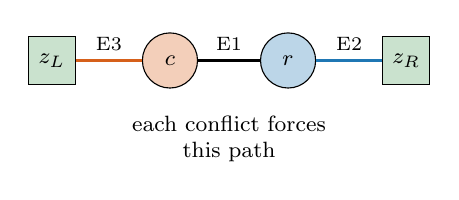
\begin{tikzpicture}[ov/.style={circle,draw,inner sep=1pt,minimum size=7mm,font=\footnotesize},
  cv/.style={rectangle,draw,inner sep=1pt,minimum size=6mm,font=\footnotesize}]
  \node[cv,fill=zcol!25] (zl) at (0,0) {$z_L$};
  \node[ov,fill=famR!30] (c) at (1.5,0) {$c$};
  \node[ov,fill=famL!30] (r) at (3.0,0) {$r$};
  \node[cv,fill=zcol!25] (zr) at (4.5,0) {$z_R$};
  \draw[thick,famR] (zl) -- node[above,font=\scriptsize,black] {E3} (c);
  \draw[thick] (c) -- node[above,font=\scriptsize] {E1} (r);
  \draw[thick,famL] (r) -- node[above,font=\scriptsize,black] {E2} (zr);
  \node[font=\footnotesize,align=center] at (2.25,-1.0) {each conflict forces\\ this path};
\end{tikzpicture}
\end{column}
\end{columns}
\end{frame}

% ------------------------------------------------------------------
\begin{frame}{Proving the pruning lemma, II: two factorizations}
\begin{columns}[c]
\begin{column}{0.5\textwidth}
Variables $a_{xy},b_{xy}$ on the arcs. Four matrices:
\begin{itemize}
\item $L:\RR^{\Rf}\!\to\RR^Z$ and $A:\RR^H\!\to\RR^{\Cf}$ move the first coordinate ($a_{pi}$);
\item $B:\RR^{\Rf}\!\to\RR^H$ and $N:\RR^Z\!\to\RR^{\Cf}$ move the second ($b_{sj}$).
\end{itemize}
Both routes from $r$ to $c$ give $a_{pi}b_{sj}$ exactly on conflicts:
\[\boxed{\ NL=AB\ }\]
The conflict matrix factors through $\RR^Z$ \emph{and} through $\RR^H$.
\end{column}
\begin{column}{0.47\textwidth}
\centering
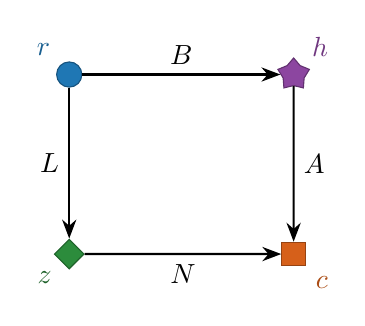
\begin{tikzpicture}[scale=0.95]
  \node[Lpt,label={[famL!80!black]above left:$r$}] (r) at (0,0) {};
  \node[Hpt,label={[hcol!80!black]above right:$h$}] (h) at (3,0) {};
  \node[Zpt,label={[zcol!70!black]below left:$z$}] (z) at (0,-2.4) {};
  \node[Rpt,label={[famR!80!black]below right:$c$}] (c) at (3,-2.4) {};
  \draw[-{Stealth[length=2.4mm]},thick] (r) -- node[left] {$L$} (z);
  \draw[-{Stealth[length=2.4mm]},thick] (z) -- node[below] {$N$} (c);
  \draw[-{Stealth[length=2.4mm]},thick] (r) -- node[above] {$B$} (h);
  \draw[-{Stealth[length=2.4mm]},thick] (h) -- node[right] {$A$} (c);
\end{tikzpicture}
\end{column}
\end{columns}
\end{frame}

% ------------------------------------------------------------------
\begin{frame}{Proving the pruning lemma, III: counting dimensions}
Take a maximum matching with the fewest conflict edges:
$k$ conflict edges, $\ell$ E2 edges, $t$ E3 edges.

\medskip
Choose \textbf{generic} real values for the variables (a finite product of
nonzero polynomials is nonzero somewhere). Then
\[
 \rank L=\ell,\qquad \rank N=t\qquad\text{(Edmonds: generic rank = matching number)}.
\]
If also $\dim\ker A\ge k$, then
\[
 \abs H=\dim\ker A+\rank A\ \ge\ k+\rank(AB)=k+\rank(NL)\ \ge\ k+\ell+t-\abs Z
\]
by Sylvester's inequality. So $\nu(\Gamma)=k+\ell+t\le\abs Z+\abs H$. \checkmark
\end{frame}

% ------------------------------------------------------------------
\begin{frame}{Proving the pruning lemma, IV: the kernel trick}
\textbf{Kernel lemma.} If $\Phi$ has maximum rank for its zero pattern $T$, then
$x\in\ker\Phi$, $y\in\ker\Phi^{\mathsf T}$ satisfy $x_jy_s=0$ for all $(s,j)\in T$.
\\{\small (Otherwise perturbing the entry $(s,j)$ would increase the rank.)}

\medskip
Applied to small blocks of $B$ and $N^{\mathsf T}$:
\[
 u\in\ker B,\ v\in\ker N^{\mathsf T},\ (r,c)\text{ conflict}\ \Longrightarrow\ u_rv_c=0.
\]
For each matched conflict edge $(r,c)$:
\begin{itemize}
\item $u^r\in\ker L$ with $u^r_r=1$ (since $r$ is not used by the E2 edges),
\item $v^c\in\ker N^{\mathsf T}$ with $v^c_c=1$.
\end{itemize}
Then $Bu^r\in\ker A$ (as $ABu^r=NLu^r=0$), and these $k$ vectors are
independent: any relation gives $u\in\ker B$ with $u_r\ne0=u_rv^c_c$.
So $\dim\ker A\ge k$.
\end{frame}

% ------------------------------------------------------------------
\begin{frame}{The main inventions}
\begin{enumerate}
\item \textbf{Upgrade to sets, then to concavity.} Minimal counterexample $\to$
subset deficit $\to$ blow-up $\to$ $\abs U+\abs{F^2U}<2\abs{FU}$, which can be
summed over lines.
\item \textbf{Lift to pairs.} Families in $X\times X$ with two independent
image operators. Compatibility is $F_1P\cap F_2Q=\varnothing$, and $(\Delta,\Delta)$ is
compatible exactly because the graph is oriented.
\item \textbf{The right potential.} Maximize $\abs P+\abs Q+\#$uncovered.
Complementing second images gains $\mu+2d$.
\item \textbf{Pruning with an outcome-dependent cost.} Pay $\abs H$ (old uncovered
points) plus the points left uncovered after pruning.
\item \textbf{Linear algebra for a matching bound.} The conflict matrix factors as
$NL=AB$, generic coefficients are used, and a kernel lemma completes the count.
\end{enumerate}
\end{frame}

% ------------------------------------------------------------------
\begin{frame}{Consequences}
\begin{itemize}
\item \textbf{Weighted forms} (Seacrest's equivalences): for every weighting
$\eta\ge0$ some $v$ has $\eta(\Nout(v))\le\eta(\Ntwo(v))$. Also, some probability
weighting works for all $v$ at once (Farkas), and there is an arc-weighted
version.
\item \textbf{Directed triangles.} With no directed triangle,
$\Ntwo(v)\subseteq$ non-neighbors, so some $v$ has $n-1\ge2d^+(v)+d^-(v)$.
\begin{itemize}
\item $\delta^+,\delta^-\ge n/3\ \Rightarrow$ a directed triangle exists;
\item $r$-regular with directed girth $4$ $\Rightarrow$ $n\ge3r+1$.
\end{itemize}
\end{itemize}
\vfill
\begin{block}{Formal verification}
The entire proof, including the pruning lemma, is formalized in Lean~4 + Mathlib
(\texttt{Seymour.seymour\_second\_neighbourhood}), with no \texttt{sorry} and only
the standard axioms.
\end{block}
\centering\small The full write-up, with figures and all details, is in the accompanying paper.
\end{frame}

\end{document}
